\documentclass{standalone}
\usepackage{tikz}
\usetikzlibrary{patterns, positioning}


\begin{document}
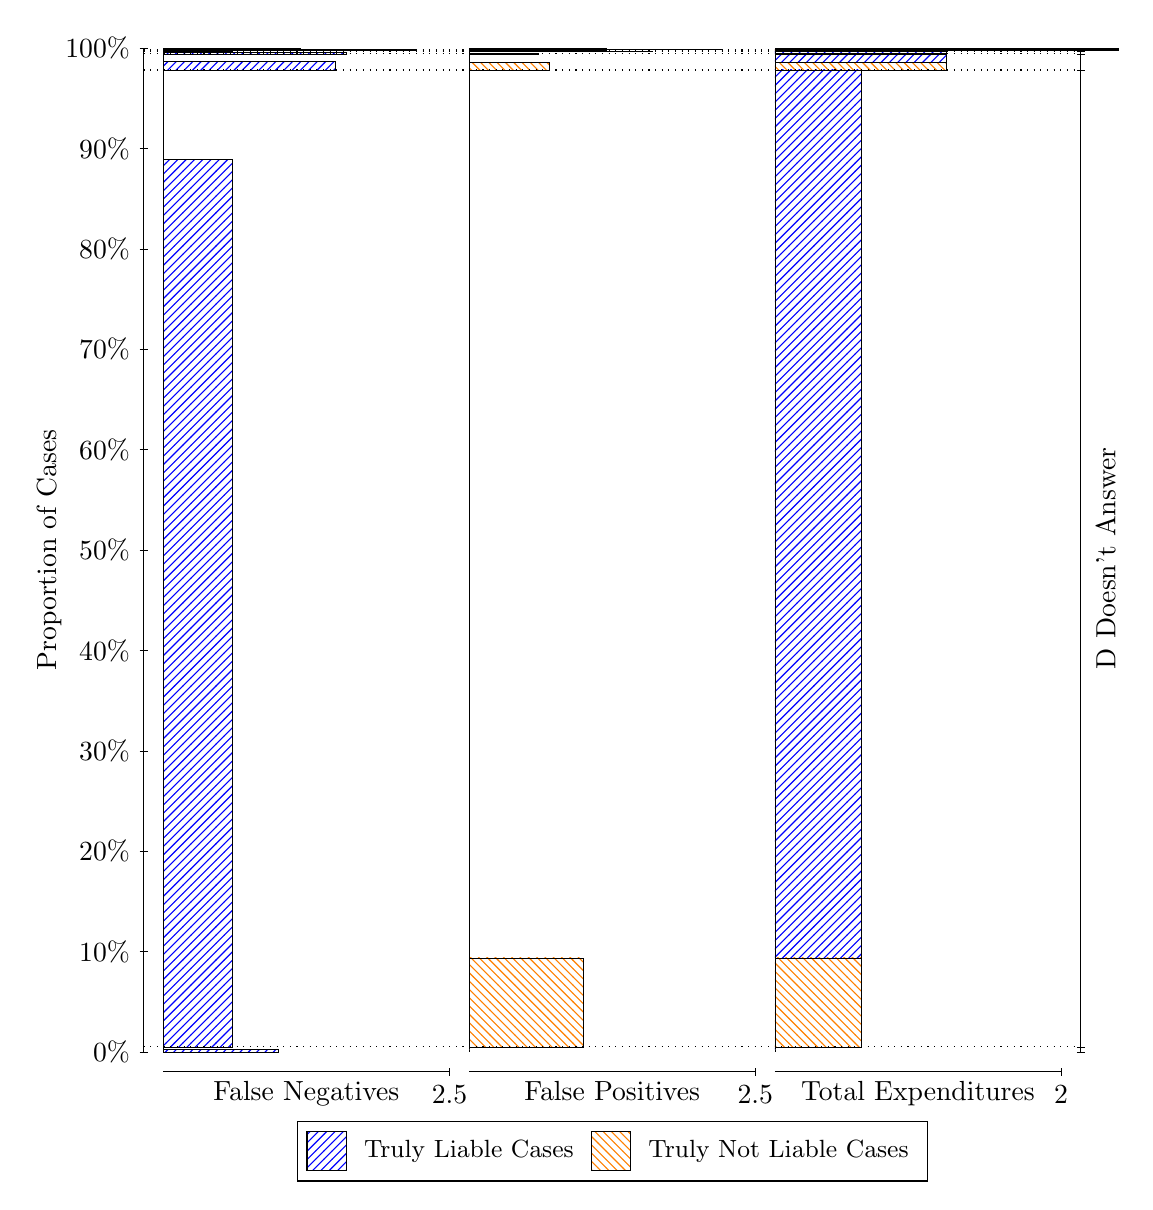
\begin{tikzpicture}
\draw[black, very thin] (1.5,1.75) -- (1.5,14.5);
\node[rotate=90, text=black, anchor=center] at (0.3, 8.125) {Proportion of Cases};
\draw[black, very thin] (1.45,1.75) -- (1.55,1.75);
\node[text=black, anchor=east] at (1.45, 1.75) {0\%};
\draw[black, very thin] (1.45,3.025) -- (1.55,3.025);
\node[text=black, anchor=east] at (1.45, 3.025) {10\%};
\draw[black, very thin] (1.45,4.3) -- (1.55,4.3);
\node[text=black, anchor=east] at (1.45, 4.3) {20\%};
\draw[black, very thin] (1.45,5.575) -- (1.55,5.575);
\node[text=black, anchor=east] at (1.45, 5.575) {30\%};
\draw[black, very thin] (1.45,6.85) -- (1.55,6.85);
\node[text=black, anchor=east] at (1.45, 6.85) {40\%};
\draw[black, very thin] (1.45,8.125) -- (1.55,8.125);
\node[text=black, anchor=east] at (1.45, 8.125) {50\%};
\draw[black, very thin] (1.45,9.4) -- (1.55,9.4);
\node[text=black, anchor=east] at (1.45, 9.4) {60\%};
\draw[black, very thin] (1.45,10.675) -- (1.55,10.675);
\node[text=black, anchor=east] at (1.45, 10.675) {70\%};
\draw[black, very thin] (1.45,11.95) -- (1.55,11.95);
\node[text=black, anchor=east] at (1.45, 11.95) {80\%};
\draw[black, very thin] (1.45,13.225) -- (1.55,13.225);
\node[text=black, anchor=east] at (1.45, 13.225) {90\%};
\draw[black, very thin] (1.45,14.5) -- (1.55,14.5);
\node[text=black, anchor=east] at (1.45, 14.5) {100\%};

\draw[black, very thin] (13.4,1.75) -- (13.4,14.5);
\draw[black, very thin] (13.35,1.75) -- (13.45,1.75);
\node[anchor=west] at (13.35, 1.75) {};
\draw[black, very thin] (13.35,1.8145) -- (13.45,1.8145);
\node[anchor=west] at (13.35, 1.8145) {};
\draw[black, very thin] (13.35,14.221) -- (13.45,14.221);
\node[anchor=west] at (13.35, 14.221) {};
\draw[black, very thin] (13.35,14.425) -- (13.45,14.425);
\node[anchor=west] at (13.35, 14.425) {};
\draw[black, very thin] (13.35,14.453) -- (13.45,14.453);
\node[anchor=west] at (13.35, 14.453) {};
\draw[black, very thin] (13.35,14.469) -- (13.45,14.469);
\node[anchor=west] at (13.35, 14.469) {};
\draw[black, very thin] (13.35,14.484) -- (13.45,14.484);
\node[anchor=west] at (13.35, 14.484) {};
\draw[black, very thin] (13.35,14.5) -- (13.45,14.5);
\node[anchor=west] at (13.35, 14.5) {};

\draw[black, very thin, pattern color=blue, pattern=north east lines] (1.75,1.75) rectangle (3.2033,1.7832);
\draw[black, very thin, pattern color=orange, pattern=north west lines] (1.75,1.7832) rectangle (1.75,1.8145);
\draw[black, very thin, pattern color=blue, pattern=north east lines] (1.75,1.8145) rectangle (2.622,13.09);
\draw[black, very thin, pattern color=orange, pattern=north west lines] (1.75,13.09) rectangle (1.75,14.221);
\draw[black, very thin, pattern color=blue, pattern=north east lines] (1.75,14.221) rectangle (3.93,14.326);
\draw[black, very thin, pattern color=orange, pattern=north west lines] (1.75,14.326) rectangle (1.75,14.425);
\draw[black, very thin, pattern color=blue, pattern=north east lines] (1.75,14.425) rectangle (4.0753,14.445);
\draw[black, very thin, pattern color=orange, pattern=north west lines] (1.75,14.445) rectangle (1.75,14.453);
\draw[black, very thin, pattern color=blue, pattern=north east lines] (1.75,14.453) rectangle (2.622,14.468);
\draw[black, very thin, pattern color=orange, pattern=north west lines] (1.75,14.468) rectangle (1.75,14.469);
\draw[black, very thin, pattern color=blue, pattern=north east lines] (1.75,14.469) rectangle (4.9473,14.481);
\draw[black, very thin, pattern color=orange, pattern=north west lines] (1.75,14.481) rectangle (1.75,14.484);
\draw[black, very thin, pattern color=blue, pattern=north east lines] (1.75,14.484) rectangle (3.494,14.499);
\draw[black, very thin, pattern color=orange, pattern=north west lines] (1.75,14.499) rectangle (1.75,14.5);
\draw[black, very thin, pattern color=orange, pattern=north west lines] (5.6333,1.75) rectangle (5.6333,1.7814);
\draw[black, very thin, pattern color=blue, pattern=north east lines] (5.6333,1.7814) rectangle (5.6333,1.8145);
\draw[black, very thin, pattern color=orange, pattern=north west lines] (5.6333,1.8145) rectangle (7.0867,2.9451);
\draw[black, very thin, pattern color=blue, pattern=north east lines] (5.6333,2.9451) rectangle (5.6333,14.221);
\draw[black, very thin, pattern color=orange, pattern=north west lines] (5.6333,14.221) rectangle (6.6507,14.319);
\draw[black, very thin, pattern color=blue, pattern=north east lines] (5.6333,14.319) rectangle (5.6333,14.425);
\draw[black, very thin, pattern color=orange, pattern=north west lines] (5.6333,14.425) rectangle (6.5053,14.433);
\draw[black, very thin, pattern color=blue, pattern=north east lines] (5.6333,14.433) rectangle (5.6333,14.453);
\draw[black, very thin, pattern color=orange, pattern=north west lines] (5.6333,14.453) rectangle (7.9587,14.455);
\draw[black, very thin, pattern color=blue, pattern=north east lines] (5.6333,14.455) rectangle (6.5053,14.469);
\draw[black, very thin, pattern color=orange, pattern=north west lines] (5.6333,14.469) rectangle (7.3773,14.472);
\draw[black, very thin, pattern color=blue, pattern=north east lines] (5.6333,14.472) rectangle (5.924,14.484);
\draw[black, very thin, pattern color=orange, pattern=north west lines] (5.6333,14.484) rectangle (8.8307,14.485);
\draw[black, very thin, pattern color=blue, pattern=north east lines] (5.6333,14.485) rectangle (7.3773,14.5);
\draw[black, very thin, pattern color=orange, pattern=north west lines] (9.5167,1.75) rectangle (9.5167,1.7814);
\draw[black, very thin, pattern color=blue, pattern=north east lines] (9.5167,1.7814) rectangle (9.5167,1.8145);
\draw[black, very thin, pattern color=orange, pattern=north west lines] (9.5167,1.8145) rectangle (10.607,2.9451);
\draw[black, very thin, pattern color=blue, pattern=north east lines] (9.5167,2.9451) rectangle (10.607,14.221);
\draw[black, very thin, pattern color=orange, pattern=north west lines] (9.5167,14.221) rectangle (11.697,14.319);
\draw[black, very thin, pattern color=blue, pattern=north east lines] (9.5167,14.319) rectangle (11.697,14.425);
\draw[black, very thin, pattern color=orange, pattern=north west lines] (9.5167,14.425) rectangle (11.697,14.433);
\draw[black, very thin, pattern color=blue, pattern=north east lines] (9.5167,14.433) rectangle (11.697,14.453);
\draw[black, very thin, pattern color=orange, pattern=north west lines] (9.5167,14.453) rectangle (11.697,14.455);
\draw[black, very thin, pattern color=blue, pattern=north east lines] (9.5167,14.455) rectangle (11.697,14.469);
\draw[black, very thin, pattern color=orange, pattern=north west lines] (9.5167,14.469) rectangle (13.877,14.472);
\draw[black, very thin, pattern color=blue, pattern=north east lines] (9.5167,14.472) rectangle (13.877,14.484);
\draw[black, very thin, pattern color=orange, pattern=north west lines] (9.5167,14.484) rectangle (13.877,14.485);
\draw[black, very thin, pattern color=blue, pattern=north east lines] (9.5167,14.485) rectangle (13.877,14.5);
\draw[black, dotted] (1.5,1.8145) -- (13.4,1.8145);
\draw[black, dotted] (1.5,14.221) -- (13.4,14.221);
\draw[black, dotted] (1.5,14.425) -- (13.4,14.425);
\draw[black, dotted] (1.5,14.453) -- (13.4,14.453);
\draw[black, dotted] (1.5,14.469) -- (13.4,14.469);
\draw[black, dotted] (1.5,14.484) -- (13.4,14.484);
\draw[black, very thin] (1.75,1.5) -- (5.3833,1.5);
\node[text=black, anchor=north] at (3.5667, 1.5) {False Negatives};
\draw[black, very thin] (5.3833,1.45) -- (5.3833,1.55);
\node[text=black, anchor=north] at (5.3833, 1.45) {2.5};

\draw[black, very thin] (5.6333,1.5) -- (9.2667,1.5);
\node[text=black, anchor=north] at (7.45, 1.5) {False Positives};
\draw[black, very thin] (9.2667,1.45) -- (9.2667,1.55);
\node[text=black, anchor=north] at (9.2667, 1.45) {2.5};

\draw[black, very thin] (9.5167,1.5) -- (13.15,1.5);
\node[text=black, anchor=north] at (11.333, 1.5) {Total Expenditures};
\draw[black, very thin] (13.15,1.45) -- (13.15,1.55);
\node[text=black, anchor=north] at (13.15, 1.45) {2};


\node[text=black, centered, rotate=90] at (13.72, 8.0177) {D Doesn't Answer};






\draw (7.449999999999999,1.5) node[draw=none] (baseCoordinate) {};
\begin{scope}[align=center]
        \matrix[scale=0.5, draw=black, below=0.5cm of baseCoordinate, nodes={draw}, column sep=0.1cm]{
            \node[rectangle, draw, minimum width=0.5cm, minimum height=0.5cm, pattern color=blue, pattern=north east lines] {}; &
            \node[draw=none, font=\small, text=black] (B) {Truly Liable Cases}; &
            \node[rectangle, draw, minimum width=0.5cm, minimum height=0.5cm, pattern color=orange, pattern=north west lines] {}; &
            \node[draw=none, font=\small, text=black] (B) {Truly Not Liable Cases}; \\
            };
\end{scope}

\end{tikzpicture}
\end{document}